\documentclass[tikz,border=8pt]{standalone}
% Shared look for every TikZ diagram. Load with % Shared look for every TikZ diagram. Load with % Shared look for every TikZ diagram. Load with \input{../../tools/tikz-style.tex}
\usepackage[T1]{fontenc}
\usepackage{lmodern}
\renewcommand{\sfdefault}{lmr}  % diagrams use the same serif as the text
\usetikzlibrary{arrows.meta, positioning, shapes.geometric, calc, fit, backgrounds}
\definecolor{cblue}{HTML}{4C78A8}
\definecolor{corange}{HTML}{F58518}
\definecolor{cgreen}{HTML}{54A24B}
\definecolor{cred}{HTML}{E45756}
\definecolor{cpurple}{HTML}{B279A2}
\definecolor{cgrey}{HTML}{6B6B6B}
\tikzset{
  every picture/.style={font=\sffamily, line width=1.2pt},
  box/.style={draw=#1, fill=#1!12, rounded corners=4pt, align=center, inner sep=7pt, minimum height=1.1cm},
  box/.default=cgrey,
  arrow/.style={-{Stealth[length=3mm]}, draw=cgrey, line width=1.4pt},
  title/.style={font=\sffamily\bfseries\Large},
  note/.style={font=\sffamily\small, text=cgrey, align=center},
}
\AtBeginDocument{\hyphenpenalty=10000 \exhyphenpenalty=10000}

\usepackage[T1]{fontenc}
\usepackage{lmodern}
\renewcommand{\sfdefault}{lmr}  % diagrams use the same serif as the text
\usetikzlibrary{arrows.meta, positioning, shapes.geometric, calc, fit, backgrounds}
\definecolor{cblue}{HTML}{4C78A8}
\definecolor{corange}{HTML}{F58518}
\definecolor{cgreen}{HTML}{54A24B}
\definecolor{cred}{HTML}{E45756}
\definecolor{cpurple}{HTML}{B279A2}
\definecolor{cgrey}{HTML}{6B6B6B}
\tikzset{
  every picture/.style={font=\sffamily, line width=1.2pt},
  box/.style={draw=#1, fill=#1!12, rounded corners=4pt, align=center, inner sep=7pt, minimum height=1.1cm},
  box/.default=cgrey,
  arrow/.style={-{Stealth[length=3mm]}, draw=cgrey, line width=1.4pt},
  title/.style={font=\sffamily\bfseries\Large},
  note/.style={font=\sffamily\small, text=cgrey, align=center},
}
\AtBeginDocument{\hyphenpenalty=10000 \exhyphenpenalty=10000}

\usepackage[T1]{fontenc}
\usepackage{lmodern}
\renewcommand{\sfdefault}{lmr}  % diagrams use the same serif as the text
\usetikzlibrary{arrows.meta, positioning, shapes.geometric, calc, fit, backgrounds}
\definecolor{cblue}{HTML}{4C78A8}
\definecolor{corange}{HTML}{F58518}
\definecolor{cgreen}{HTML}{54A24B}
\definecolor{cred}{HTML}{E45756}
\definecolor{cpurple}{HTML}{B279A2}
\definecolor{cgrey}{HTML}{6B6B6B}
\tikzset{
  every picture/.style={font=\sffamily, line width=1.2pt},
  box/.style={draw=#1, fill=#1!12, rounded corners=4pt, align=center, inner sep=7pt, minimum height=1.1cm},
  box/.default=cgrey,
  arrow/.style={-{Stealth[length=3mm]}, draw=cgrey, line width=1.4pt},
  title/.style={font=\sffamily\bfseries\Large},
  note/.style={font=\sffamily\small, text=cgrey, align=center},
}
\AtBeginDocument{\hyphenpenalty=10000 \exhyphenpenalty=10000}

\begin{document}
% Section 5: one function, two calls. attention(S, H, H) relates two sequences (3 x 4 weights);
% attention(Q, K, V) relates one sentence to itself (4 x 4 weights).
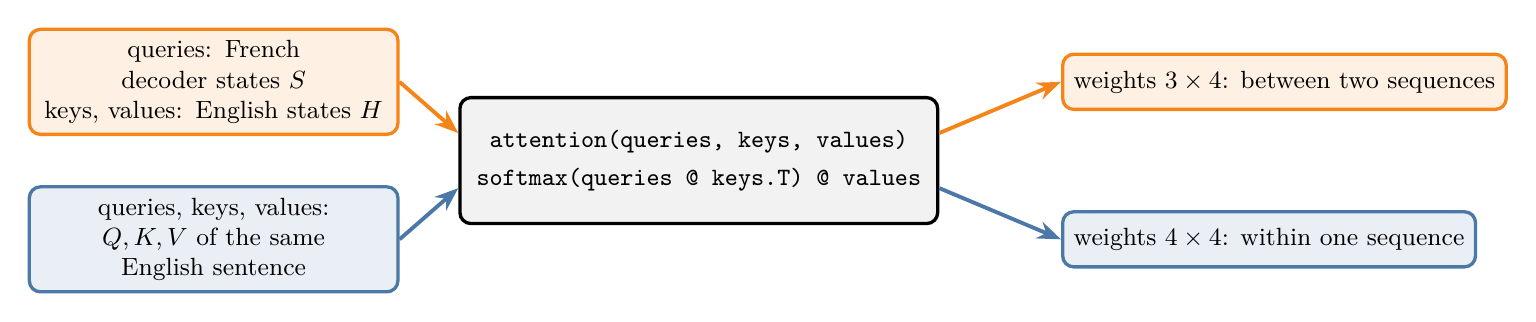
\begin{tikzpicture}[in/.style={box=#1, minimum height=0.7cm, inner sep=4pt, font=\sffamily\small, text width=4.4cm},
  f/.style={draw=black, fill=black!5, rounded corners=4pt, font=\ttfamily\small, align=center, inner sep=6pt, minimum height=1.6cm},
  out/.style={box=#1, minimum height=0.7cm, inner sep=4pt, font=\sffamily\small}]
  \node[f] (fn) at (6.0, 0) {attention(queries, keys, values)\\[3pt]softmax(queries @ keys.T) @ values};
  \node[in=corange, anchor=east] (a) at (2.2, 1.0) {queries: French decoder states $S$\\keys, values: English states $H$};
  \node[in=cblue, anchor=east] (b) at (2.2, -1.0) {queries, keys, values:\\$Q, K, V$ of the same English sentence};
  \draw[arrow, draw=corange] (a.east) -- (fn.west |- 0, 0.35);
  \draw[arrow, draw=cblue] (b.east) -- (fn.west |- 0, -0.35);
  \node[out=corange, anchor=west] (oa) at (10.6, 1.0) {weights $3 \times 4$: between two sequences};
  \node[out=cblue, anchor=west] (ob) at (10.6, -1.0) {weights $4 \times 4$: within one sequence};
  \draw[arrow, draw=corange] (fn.east |- 0, 0.35) -- (oa.west);
  \draw[arrow, draw=cblue] (fn.east |- 0, -0.35) -- (ob.west);
\end{tikzpicture}
\end{document}
